%&formules
\documentclass[presentatie.tex]{subfiles}

\begin{document}

\section{Formules}

\clearrecentlist
    
% \begin{frame}{Formules}
% 	\begin{enumerate}
% 		\item Inline
% 		\item Superscript, subscript, summation
% 		\item Equation
% 		\item Align
% 		\item Nummering
% 		\item Displaystyle vs textstyle
% 		\item (Larger)
% 	\end{enumerate}
% \end{frame}



\begin{saveblock}{formDocFrag}
	\begin{highlightblock}[gobble=8,linewidth=25em,framexleftmargin=0.25em]
		De trigonometrische identiteit
		is $ \sin^2(\theta) + \cos^2(\theta) = 1 $.
	\end{highlightblock}
\end{saveblock}

\begin{frame}{Formules}
	\centering
	\adjustbox{cfbox=red!80!black 1.5pt 3pt}{
		De trigonometrische identiteit is $ \sin^2(\theta) + \cos^2(\theta) = 1 $.
	}
	
	\vspace{10pt}
	\begin{center}%
		\adjustbox{set height=2cm,margin=2px}{%
			\only<2->{\useblock{formDocFrag}}%
		}%
	\end{center}
	
\end{frame}

\def\extraslistsep{\hspace{0.5em}\textcolor{red!80!black}{\vrule width 1pt height 0.6\baselineskip\relax}\hspace{0.5em}}
\def\es#1{\adjustbox{scale=0.8}{#1}}

\begin{frame}{Formules}%
	\renewcommand{\arraystretch}{1.5}%
	\begin{tabularx}{0.5\textwidth}{ll}
		\toprule
		Formule {\global\showcount=1\relax}& Code\\
		\midrule
		\showformula{$ \sqrt{2} $}{\\sqrt\{2\}}\\
		\showformula{$ \frac{2}{3} $}{\\frac\{2\}\{3\}}\\
		\showformula{$ 6\geq 3 $}{6\\geq 3}\\
		\showformula{$ a^2 + b^2 $}{a^2 + b^2}\\
		\bottomrule
	\end{tabularx}%
	\begin{tabularx}{0.5\textwidth}{ll}
		\toprule
		Formule {\global\showcount=5\relax}& Code\\
		\midrule
		\showformula{$ \sqrt[3]{8} $}{\\sqrt[3]\{8\}}\\
		%\showformula{$ x_1 + \dots + x_n $}{x_1 + \\dots + x_n}\\
		\showformula{$ x_1 $}{x_1}\\
		\showformula{$ x_1^2 $}{x_1^2}\\
		\showformula{$ a^{2+b^2} $}{a^\{2 + b^2\}}\\
		%\showformula{$ f(\{3, 6\}) $}{f(\\\{3, 6\\\})}\\
		\bottomrule
	\end{tabularx}%
	\par\addvspace{0.5\baselineskip}
	\unless\ifishandout
		% \only<4>{
		% 	\es{$ 3\leq 6 $}: \hll|$ 3\\leq 6 $|\extraslistsep
		% 	\es{$ 3 < 6 $}: \hll|$ 3 < 6 $|\extraslistsep
		% 	\es{$ 6 > 3 $}: \hll|$ 6 > 3 $|\extraslistsep\\
		% 	\es{$ 3\ll 6000 $}: \hll|$ 3\\ll 6000 $|\extraslistsep
		% 	\es{$ 6000\gg 3 $}: \hll|$ 6000\\gg 3 $|
		% }%
		\only<10->{
			\hll|$ x^22 $|\,: \es{$ x^22 $}
			\only<11->{\extraslistsep\hll|$ x^\{22\} $|\,: \es{$ x^{22} $}}
			\only<12->{\extraslistsep\hll|$ \{x + 3^\{2\}\} \{\} + 9 $|\,: \es{$ {x + 3^{2}} {} + 9 $}}
		}%
	\fi
\end{frame}


\begin{frame}{Formules}%
	\renewcommand{\arraystretch}{1.5}%
	\begin{tabularx}{0.6\textwidth}{ll}
		\toprule
		Formule {\global\showcount=1\relax}& Code\\
		\midrule
		\showformula{$ x_1,\dots,x_n $}{x_1,\\dots,x_n}\\
		\showformula{$ \alpha,\beta,\gamma $}{\\alpha,\\beta,\\gamma}\\
		\showformula{$ \epsilon,\varepsilon $}{\\epsilon,\\varepsilon}\\
		\showformula{$ \phi,\varphi $}{\\phi,\\varphi}\\
		\bottomrule
	\end{tabularx}%
	\begin{tabularx}{0.4\textwidth}{ll}
		\toprule
		Formule {\global\showcount=5\relax}& Code\\
		\midrule
		\showformula{$ 5\cdot 6 $}{5\\cdot 6}\\
		%\showformula{$ x_1 + \dots + x_n $}{x_1 + \\dots + x_n}\\
		\showformula{$ A,B,\Gamma $}{A,B,\\Gamma}\\
		\showformula{$ \mathcal{P} $}{\\mathcal\{P\}}\\
		\showformula{$ \mathbb{P} $}{\\mathbb\{P\}}\\
		%\showformula{$ f(\{3, 6\}) $}{f(\\\{3, 6\\\})}\\
		\bottomrule
	\end{tabularx}%
	\par\addvspace{0.5\baselineskip}
	\unless\ifishandout
		% \only<4>{
		% 	\es{$ 3\leq 6 $}: \hll|$ 3\\leq 6 $|\extraslistsep
		% 	\es{$ 3 < 6 $}: \hll|$ 3 < 6 $|\extraslistsep
		% 	\es{$ 6 > 3 $}: \hll|$ 6 > 3 $|\extraslistsep\\
		% 	\es{$ 3\ll 6000 $}: \hll|$ 3\\ll 6000 $|\extraslistsep
		% 	\es{$ 6000\gg 3 $}: \hll|$ 6000\\gg 3 $|
		% }%
		% \only<10->{
		% 	\hll|$ x^22 $|\,: \es{$ x^22 $}
		% 	\only<11->{\extraslistsep\hll|$ x^\{22\} $|\,: \es{$ x^{22} $}}
		% 	\only<12->{\extraslistsep\hll|$ \{x + 3^\{2\}\} \{\} + 9 $|\,: \es{$ {x + 3^{2}} {} + 9 $}}
		% }%
	\fi
\end{frame}



\begin{frame}
	
	\begin{align*}
		\nabla\times(\nabla\times\mathbf{A}) = \nabla(\nabla\cdot \mathbf{A}) - \nabla^2\mathbf{A}
	\end{align*}
\end{frame}

\begin{frame}
	
	\begin{equation*}
		\alpha,\beta,\gamma,\delta,\epsilon,\zeta,\eta,\theta,\iota,\kappa,\lambda,
		\mu,\nu,\xi,o,\pi,\rho,\sigma,\tau,\upsilon,\phi,\chi,\psi,\omega
	\end{equation*}
	\begin{equation*}
		A,B,\Gamma,\Delta,E,Z,H,\Theta,I,K,\Lambda,
		M,N,\Xi,O,\Pi,P,\Sigma,T,\Upsilon,\Phi,\chi,\Psi,\Omega
	\end{equation*}
	\begin{equation*}
		\varDelta,\varepsilon,\varGamma,\varkappa,\varLambda,%\varnothing,
		\varOmega,\varPhi,\varphi,\varPi,\varpi,%\varpropto,
		\varPsi,\varrho,
		\varSigma,\varsigma,\varTheta,\vartheta,%\vartriangle,
		\varUpsilon,\varXi
	\end{equation*}

	
	\begin{equation}
		\mathbb{P}, \mathcal{C}
	\end{equation}
	
	\begin{equation}
		\forall, \exists, \lnot, \land, \lor, \wedge, \hat{\imath}, \hat{n}, \vec{F}_{\text{tot}},
		\frac{\partial f}{\partial x}, \frac{\dif f}{\dif y}, %\left A\dfrac{2}{3}\middle B\right C
	\end{equation}
	% \DeclareMathOperator{\test}{test}
\end{frame}

\begin{frame}{Wiskundige relaties}
	\renewcommand{\arraystretch}{1.5}%
	\begin{tabularx}{0.5\textwidth}{ll}
		\toprule
		Formule {\global\showcount=1\relax}& Code\\
		\midrule
		\showformulaa{$ a\leq b $}{a \\leq b}\\
		\showformulaa{$ a < b  $}{a < b}\\
		\showformulaa{$ a\ll b $}{a \\ll b}\\
		\showformulaa{$ a = b $}{a = b}\\
		\showformulaa{$ a \neq b $}{a \\neq b}\\
		\showformulaa{$ a\sim b  $}{a \\sim b}\\
		\bottomrule
	\end{tabularx}%
	\begin{tabularx}{0.5\textwidth}{ll}
		\toprule
		Formule {\global\showcount=1\relax}& Code\\
		\midrule
		\showformulaa{$ a\geq b  $}{a \\geq b}\\
		\showformulaa{$ a > b $}{a > b}\\
		\showformulaa{$ a\gg b $}{a \\gg b}\\
		\showformulaa{$ a\simeq b $}{a \\simeq b}\\
		\showformulaa{$ a\approx b $}{a \\approx b}\\
		{}&{}\\
		\bottomrule
	\end{tabularx}%
\end{frame}

%\begin{frame}{Formules}
%	%\hll|$| \only<2->{\hll|\\sqrt\{2\}|}\only<-1>{??} \hll|$|
%	%\hideformula[2]{\\sqrt\{2\}}
%	%\bgroup
%	\renewcommand{\arraystretch}{1.5}
%	\begin{tabularx}{\textwidth}{ll}
%		\toprule
%		Formule {\global\showcount=1\relax}& Code\\
%		\midrule
%		\showformula{$ \sqrt{2} + \sqrt[3]{8} $}{\\sqrt\{2\} {} + \\sqrt[3]\{8\}}\\
%		\showformula{$ \frac{2}{3} $}{\\frac\{2\}\{3\}}\\
%		\showformula{$ 2 + 3^2 + 1 $}{2 + 3^2 + 1}\\
%		\showformula{$ 2 + 3^{2 + 1} $}{2 + 3^\{2 + 1\}}\\
%		\showformula{$ a_1^2 + x^23 - x^{23} $}{a_1^2 + x^23 - x^\{23\}}\\
%		\showformula{$ \sin(2\pi) + {a_1}^2 - (a_1)^2 $}{\\sin(2\\pi) + \{a_1\}^2 - (a_1)^2}\\
%		\bottomrule
%	\end{tabularx}
%	%\egroup
%\end{frame}

\updatehighlight{
	name=accentC,
	remove={},
	add={equation},
	%
	name=default,
	add={}
}

\begin{saveblock}{equation}
	\begin{highlightblock}[gobble=8,linewidth=\textwidth,
		framexleftmargin=0.25em,xleftmargin=0.25em]
		De trigonometrische identiteit is
		$ \sin^2(\theta) + \cos^2(\theta) = 1. $

		De trigonometrische identiteit is 
		\begin{equation}
			\sin^2(\theta) + \cos^2(\theta) = 1.
		\end{equation}
	\end{highlightblock}
\end{saveblock}

% Daarmee kunnen we de
% verdubbelingsformule herschrijven
% als
% \begin{align}
% 	\cos(2\theta) 
% 	&= \cos^2(\theta) 
% 		- \sin^2(\theta)\\
% 	&= 2\cos^2(\theta)-1.
% \end{align}

\addtorecentlist{equation}

\begin{frame}{Equation}

	\useblock{equation}

	\includegraphics[width=\linewidth,height=0.4\textheight,keepaspectratio]{assets/5_Formules/mathEquation.pdf}

	% \begin{columns}
	% 	\begin{column}{0.6\textwidth}
	% 		\useblock{equation}
	% 	\end{column}
	% 	\begin{column}{0.5\textwidth}
	% 		\includegraphics[width=\linewidth,height=0.8\textheight,keepaspectratio]{assets/mathEquation.pdf}
	% 	\end{column}
	% \end{columns}
\end{frame}

\updatehighlight{
	name=accentC,
	remove={equation},
	add={align},
	%
	name=default,
	add={}
}

\begin{saveblock}{align}
	\begin{highlightblock}[gobble=8,linewidth=\textwidth,
		framexleftmargin=0.25em,xleftmargin=0.25em]
		De verdubbelingsformule herschrijven we nu als
		\begin{align}
			\cos(2\theta) = \cos^2(\theta) - \sin^2(\theta)\\
			= 2\cos^2(\theta)-1.
		\end{align}
	\end{highlightblock}
\end{saveblock}

\addtorecentlist{align}

\begin{frame}{Align}
	\useblock{align}

	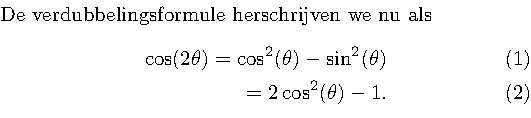
\includegraphics[width=\linewidth,height=0.4\textheight,keepaspectratio]{assets/5_Formules/mathAlignUnaligned.pdf}
\end{frame}

\begin{saveblock}{align}
	\begin{highlightblock}[gobble=8,linewidth=\textwidth,
		framexleftmargin=0.25em,xleftmargin=0.25em]
		De verdubbelingsformule herschrijven we nu als
		\begin{align}
			\cos(2\theta) &= \cos^2(\theta) - \sin^2(\theta)\\
			&= 2\cos^2(\theta)-1.
		\end{align}
	\end{highlightblock}
\end{saveblock}

\begin{frame}{Align}
	\useblock{align}

	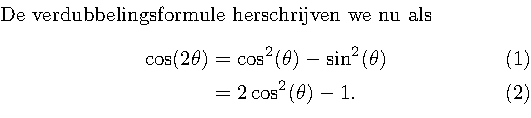
\includegraphics[width=\linewidth,height=0.4\textheight,keepaspectratio]{assets/5_Formules/mathAlignDoubleNumber.pdf}
\end{frame}

\updatehighlight{
	name=accentC,
	remove={align},
	add={\nonumber},
	%
	name=default,
	add={},
	%
	name=accentBlack,
	color=black,
	add={align}
}

\begin{saveblock}{align}
	\begin{highlightblock}[gobble=8,linewidth=\textwidth,
		framexleftmargin=0.25em,xleftmargin=0.25em]
		De verdubbelingsformule herschrijven we nu als
		\begin{align}
			\cos(2\theta) &= \cos^2(\theta) - \sin^2(\theta)
			\nonumber\\
			&= 2\cos^2(\theta)-1.
		\end{align}
	\end{highlightblock}
\end{saveblock}

\addtorecentlist{\textbackslash nonumber}

\begin{frame}{Align}
	\useblock{align}

	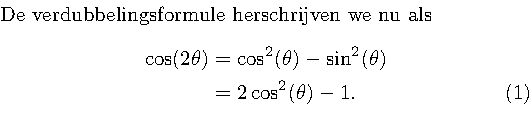
\includegraphics[width=\linewidth,height=0.4\textheight,keepaspectratio]{assets/5_Formules/mathAlignSecondNumbered.pdf}
\end{frame}

\updatehighlight{
	name=accentC,
	remove={\nonumber},
	add={*},
	%
	name=default,
	add={\nonumber}
}

\begin{saveblock}{align}
	\begin{highlightblock}[gobble=8,linewidth=\textwidth,
		framexleftmargin=0.25em,xleftmargin=0.25em]
		De verdubbelingsformule herschrijven we nu als
		\begin{align*}
			\cos(2\theta) &= \cos^2(\theta) - \sin^2(\theta)\\
			&= 2\cos^2(\theta)-1.
		\end{align*}
	\end{highlightblock}
\end{saveblock}

\addtorecentlist{align*}

\begin{frame}{Align}
	\useblock{align}

	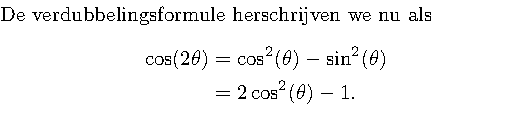
\includegraphics[width=\linewidth,height=0.4\textheight,keepaspectratio]{assets/5_Formules/mathAlignNoNumbers.pdf}
\end{frame}

\updatehighlight{
	name=accentC,
	add={\tag},
	remove={*},
	%
	name=accentBlack,
	color=black,
	add={*}
}

\addtorecentlist{\textbackslash tag}

\begin{saveblock}{align}
	\begin{highlightblock}[gobble=8,linewidth=\textwidth,
		framexleftmargin=0.25em,xleftmargin=0.25em]
		De verdubbelingsformule herschrijven we nu als
		\begin{align*}
			\cos(2\theta) &= \cos^2(\theta) - \sin^2(\theta)\\
			&= 2\cos^2(\theta)-1. \tag{Alt. verd. form.}
		\end{align*}
	\end{highlightblock}
\end{saveblock}

\begin{frame}{Align}
	\useblock{align}

	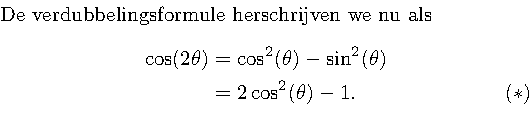
\includegraphics[width=\linewidth,height=0.4\textheight,keepaspectratio]{assets/5_Formules/mathTag.pdf}
\end{frame}


\begin{saveblock}{align}
	\begin{highlightblock}[gobble=8,linewidth=\textwidth,
		framexleftmargin=0.25em,xleftmargin=0.25em]
		Dit doen we met de verdubbelingsformule
		\begin{align}
			\cos(2\theta) &= \cos^2(\theta) - \sin^2(\theta),
		\end{align}
		die we kunnen herschrijven als
		\begin{align}
			&= \cos^2(\theta) - (1 - \cos^2(\theta))\\
			&= 2\cos^2(\theta)-1.
		\end{align}
	\end{highlightblock}
\end{saveblock}

\begin{frame}{Align}
	\useblock{align}

	\centering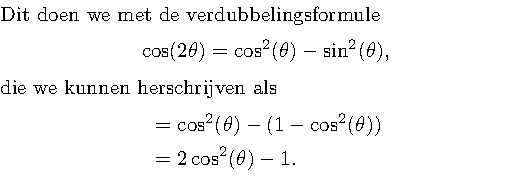
\includegraphics[width=\linewidth,height=0.3\textheight,keepaspectratio]{assets/5_Formules/mathAlignBroken.pdf}
\end{frame}


\begin{saveblock}{align}
	\begin{highlightblock}[gobble=8,linewidth=\textwidth,
		framexleftmargin=0.25em,xleftmargin=0.25em]
		Dit doen we met de verdubbelingsformule
		\begin{align}
			\cos(2\theta) &= \cos^2(\theta) - \sin^2(\theta),
		\intertext{die we kunnen herschrijven als}
			&= \cos^2(\theta) - (1 - \cos^2(\theta))\\
			&= 2\cos^2(\theta)-1.
		\end{align}
	\end{highlightblock}
\end{saveblock}

\addtorecentlist{\textbackslash intertext}

\begin{frame}{Align}
	\useblock{align}

	\centering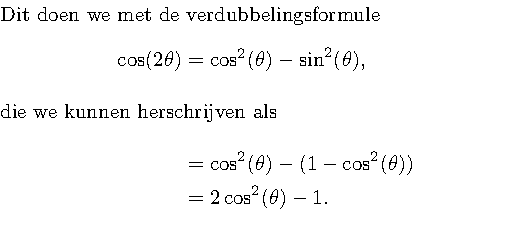
\includegraphics[width=\linewidth,height=0.4\textheight,keepaspectratio]{assets/5_Formules/mathAlignIntertext.pdf}
\end{frame}

\begin{saveblock}{otherMathNotations}
	\begin{highlightblock}[gobble=8,linewidth=0.5\textwidth,
		framexleftmargin=0.25em,xleftmargin=0.25em]
		AA \(\sqrt{2}\)
		BB \[\sqrt{3}\]
		CC $$ \sqrt{4} $$
	\end{highlightblock}
\end{saveblock}

\addtorecentlist{\textbackslash [ \textellipsis\textbackslash]}

\begin{frame}{Ook in gebruik}
	\begin{columns}
		\begin{column}{0.5\textwidth}
			\useblock{otherMathNotations}
		\end{column}
		\begin{column}{0.5\textwidth}
			\fbox{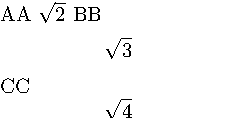
\includegraphics[width=\linewidth-2\fboxrule-2\fboxsep,height=0.9\textheight,keepaspectratio]{assets/5_Formules/mathOtherNotations.pdf}}
		\end{column}
	\end{columns}

	% \useblock{otherMathNotations}

	% 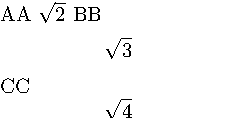
\includegraphics[width=\linewidth,height=0.4\textheight,keepaspectratio]{assets/5_Formules/mathOtherNotations.pdf}
\end{frame}


\begin{saveblock}{leftRight}
	\begin{highlightblock}[gobble=8,linewidth=\textwidth,framexleftmargin=0.25em]
		\begin{align*}
			&f(\sum~~_{i=1}^{n}x_i)\\
			&f\left(\sum~~_{i=1}^{n}x_i\right)
		\end{align*}
	\end{highlightblock}
\end{saveblock}

\begin{frame}{Left-right}
	\useblock{leftRight}

	\begin{align*}
		&f(\sum_{i=1}^{n}x_i)\\
		&f\left(\sum_{i=1}^{n}x_i\right)\\
	\end{align*}
\end{frame}

\begin{saveblock}{leftRight}
	\begin{highlightblock}[gobble=8,linewidth=\textwidth,framexleftmargin=0.25em]
		\begin{align*}
			A &= \left\{x^2\;\middle~~|\; x\in\mathbb{Z}\right\}\\
			A &= \left\{x^2\;|\; x\in\mathbb{Z}\right\}\\
			A &= \left\{x^2\mid x\in\mathbb{Z}\right\}
		\end{align*}
	\end{highlightblock}
\end{saveblock}

\begin{frame}
	\useblock{leftRight}

	\begin{align*}
		A &= \left\{x^2\;\middle|\; x\in\mathbb{Z}\right\}\\
		A &= \left\{x^2\;|\; x\in\mathbb{Z}\right\}\\
		A &= \left\{x^2\mid x\in\mathbb{Z}\right\}
	\end{align*}
\end{frame}

\begin{saveblock}{leftRight}
	\begin{highlightblock}[gobble=8,linewidth=\textwidth,framexleftmargin=0.25em]
		\begin{align*}
			\left.\left[x^2\right]\right~~|_{x=0}^{x=2} = 4,\quad
			\abs{x} = \left\{\begin{array}{ll}
				x & \mbox{if $ x \geq 0$}\\
				-x & \mbox{if $ x < 0$}
			\end{array}\right.
		\end{align*}
	\end{highlightblock}
\end{saveblock}

\begin{frame}{Delimiter point}
	\useblock{leftRight}

	\begin{align*}
		\left.\left[x^2\right]\right|_{x=0}^{x=2} = 4,\quad
		\abs{x} = \left\{\begin{array}{ll}
			x & \mbox{if $ x \geq 0$}\\
			-x & \mbox{if $ x < 0$}
		\end{array}\right.
	\end{align*}
\end{frame}

\begin{saveblock}{leftRight}
	\begin{highlightblock}[gobble=8,linewidth=\textwidth,framexleftmargin=0.25em]
		\begin{align*}
			\abs{x} = \begin{cases}
				x & \mbox{if $ x \geq 0$}\\
				-x & \mbox{if $ x < 0$}
			\end{cases}
		\end{align*}
	\end{highlightblock}
\end{saveblock}

\begin{frame}
	\useblock{leftRight}
	
	\begin{align*}
		\abs{x} = \begin{cases}
			x & \mbox{if $ x \geq 0$}\\
			-x & \mbox{if $ x < 0$}
		\end{cases}
	\end{align*}
\end{frame}

\begin{saveblock}{matrix}
	\begin{highlightblock}[gobble=8,linewidth=\textwidth,framexleftmargin=0.25em]
		\begin{align*}
			R(\theta) = \begin{pmatrix}
				\cos(\theta) & -\sin(\theta)\\
				\sin(\theta) & \cos(\theta)
			\end{pmatrix},\quad
			A = \left~~|\begin{matrix}
				4 & 3\\
				-1 & 2
			\end{matrix}\right)
		\end{align*}
	\end{highlightblock}
\end{saveblock}

\begin{frame}
	\useblock{matrix}

	\begin{align*}
		R(\theta) = \begin{pmatrix}
			\cos(\theta) & -\sin(\theta)\\
			\sin(\theta) & \cos(\theta)
		\end{pmatrix},\quad
		A = \left|\begin{matrix}
			4 & 3\\
			-1 & 2
		\end{matrix}\right)
	\end{align*}
\end{frame}

\begin{saveblock}{matrix}
	\begin{highlightblock}[gobble=8,linewidth=\textwidth,framexleftmargin=0.25em]
		\begin{align*}
			I_n = \begin{pmatrix}
				1 & 0 & \cdots & 0\\
				0 & 1 & \cdots & 0\\
				\vdots & \vdots & \ddots & \vdots\\
				0 & 0 & \cdots & 1
			\end{pmatrix}
		\end{align*}
	\end{highlightblock}
\end{saveblock}

\begin{frame}
	\useblock{matrix}

	\begin{align*}
		I_n = \begin{pmatrix}
			1 & 0 & \cdots & 0\\
			0 & 1 & \cdots & 0\\
			\vdots & \vdots & \ddots & \vdots\\
			0 & 0 & \cdots & 1
		\end{pmatrix}
	\end{align*}
\end{frame}	


\begin{frame}
	
	\begin{align*}
		\int_{x=0}^{x=\infty}e^{-x}\dif x\\
		\iint_{S}\textbf{v}\cdot\dif \textbf{S}\\
		\oint_{l}f\left(\textbf{r}\right)\dif\textbf{r}\\
		\oiint_{l}f\left(\textbf{r}\right)\dif\textbf{r}\quad \mbox{esint}
	\end{align*}
\end{frame}

\end{document}
